\subsection{UC8: Condivisione dei grafici}
\hypertarget{UC8}{}
\begin{figure} [H]
	\centering
	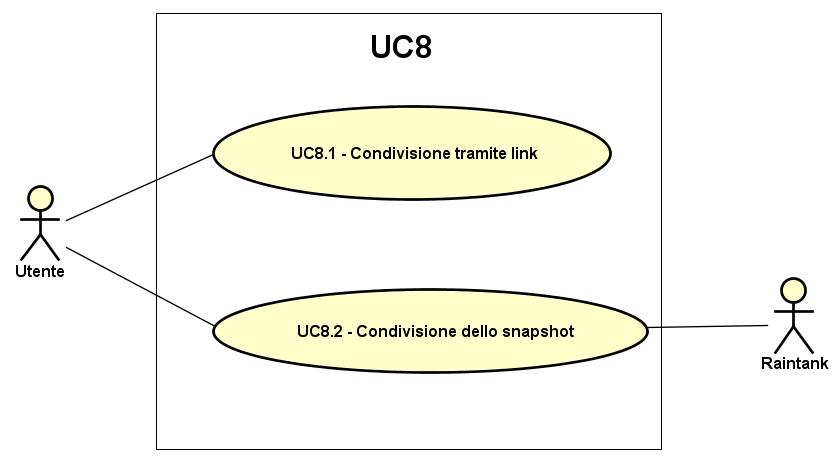
\includegraphics[scale=0.45]{Img/UC8}
	\caption{UC8 - Condivisione dei grafici}\label{}
\end{figure}
\begin{itemize}
	\item \textbf{Attori}: Utente;
	\item \textbf{Descrizione}: l'attore può condividere i grafici presenti nella dashboard;
	\item \textbf{Precondizione}: il sistema mette a disposizione diversi modi per effettuare la condivisione dei grafici;
	\item \textbf{Flusso principale degli eventi}:
	\begin{itemize}
		\item Condivisione tramite link (UC8.1);
		\item Inclusione tramite codice HTML (UC8.2);	
		\item Condivisione di snapshot.
	\end{itemize}
	\item \textbf{Postcondizione}: il grafico è stato condiviso nel modo scelto dall'attore;
	\item \textbf{Estensioni}:
	\begin{itemize}
		\item Selezione opzioni di visualizzazione (UC8.3).
	\end{itemize}
	
\end{itemize}

\subsection{UC8.1: Condivisione tramite link}
\hypertarget{UC8.1}{}
\begin{itemize}
	\item \textbf{Attori}: Utente;
	\item \textbf{Descrizione}: l'attore visualizza un link diretto alla dashboard o ad un panel;
	\item \textbf{Precondizione}: il sistema permette la visualizzazione di link per la condivisione di dashboard e panel;
	\item \textbf{Postcondizione}: Viene mostrato il link per la condivisione del grafico.
\end{itemize}

\subsection{UC8.2: Inclusione tramite codice HTML}
\hypertarget{UC8.2}{}
\begin{itemize}
	\item \textbf{Attori}: Utente;
	\item \textbf{Descrizione}: l'attore visualizza il codice \gl{HTML} per includere un panel in una pagina web;
	\item \textbf{Precondizione}: il sistema permette la visualizzazione del codice HTML per l'inclusione di panel;
	\item \textbf{Postcondizione}: viene mostrato il codice HTML per l'inclusione del panel.
\end{itemize}


\subsection{UC8.3: Selezione opzioni di visualizzazione}
\hypertarget{UC8.3}{}
\begin{figure} [H]
	\centering
	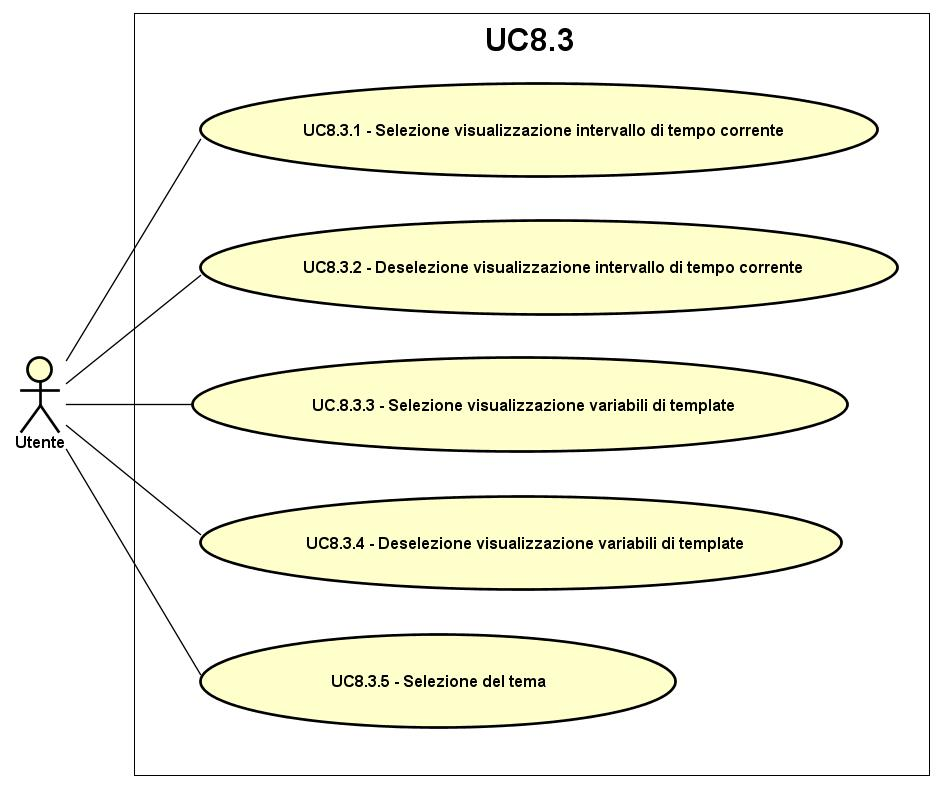
\includegraphics[scale=0.45]{Img/UC8-3}
	\caption{UC8.3 - Selezione opzioni di visualizzazione}\label{}
\end{figure}
\begin{itemize}
	\item \textbf{Attori}: Utente;
	\item \textbf{Descrizione}: l'attore può selezionare le opzioni per la visualizzazione del grafico da condividere;
	\item \textbf{Precondizione}: il sistema permette la selezione di opzioni per la visualizzazione di grafici;
	\item \textbf{Flusso principale degli eventi}:
	\begin{itemize}
		\item Selezione visualizzazione intervallo di tempo corrente (UC8.3.1);
		\item Deselezione visualizzazione intervallo di tempo corrente (UC8.3.2);
		\item Selezione visualizzazione variabili di template (8.3.3);
		\item Deselezione visualizzazione variabili di template (8.3.4);
		\item Selezione del tema (UC8.3.5).
	\end{itemize}
	\item \textbf{Postcondizione}: le opzioni di visualizzazione del grafico sono state selezionate.
\end{itemize}

\subsection{UC8.3.1: Selezione visualizzazione intervallo di tempo corrente}
\hypertarget{UC8.3.1}{}
\begin{itemize}
	\item \textbf{Attori}: Utente;
	\item \textbf{Descrizione}: l'attore seleziona la visualizzazione dell'intervallo di tempo in cui sono stati raccolti i dati presenti nel grafico;
	\item \textbf{Precondizione}: il sistema permettere di selezionare la visualizzazione dell'intervallo di tempo in un grafico;
	\item \textbf{Postcondizione}: l'intervallo di tempo in cui sono stati raccolti i dati presenti viene visualizzato nel grafico.
\end{itemize}

\subsection{UC8.3.2: Deselezione visualizzazione intervallo di tempo corrente}
\hypertarget{UC8.3.2}{}
\begin{itemize}
	\item \textbf{Attori}: Utente;
	\item \textbf{Descrizione}: l'attore deseleziona la visualizzazione dell'intervallo di tempo in cui sono stati raccolti i dati presenti nel grafico;
	\item \textbf{Precondizione}: il sistema permettere di deselezionare la visualizzazione dell'intervallo di tempo in un grafico;
	\item \textbf{Postcondizione}: l'intervallo di tempo in cui sono stati raccolti i dati presenti non viene visualizzato nel grafico.
\end{itemize}

\subsection{UC8.3.3: Selezione visualizzazione variabili di template}
\hypertarget{UC8.3.3}{}
\begin{itemize}
	\item \textbf{Attori}: Utente;
	\item \textbf{Descrizione}: l'attore seleziona la visualizzazione delle variabili di template nel grafico;
	\item \textbf{Precondizione}: il sistema permette di selezionare la visualizzazione delle variabili di template in un grafico;
	\item \textbf{Postcondizione}: le variabili di template vengono visualizzate nel grafico.
\end{itemize}

\subsection{UC8.3.4: Deselezione visualizzazione variabili di template}
\hypertarget{UC8.3.4}{}
\begin{itemize}
	\item \textbf{Attori}: Utente;
	\item \textbf{Descrizione}: l'attore deseleziona la visualizzazione delle variabili di template nel grafico;
	\item \textbf{Precondizione}: il sistema permette di deselezionare la visualizzazione delle variabili di template in un grafico;
	\item \textbf{Postcondizione}: le variabili di template non vengono visualizzate nel grafico.
\end{itemize}

\subsection{UC8.3.5: Selezione del tema}
\hypertarget{UC8.3.5}{}
\begin{itemize}
	\item \textbf{Attori}: Utente;
	\item \textbf{Descrizione}: l'attore seleziona i colori di sfondo del grafico; 
	\item \textbf{Precondizione}: il sistema permette la selezione di temi tra quelli predefiniti;
	\item \textbf{Postcondizione}: il tema del grafico viene selezionato.
\end{itemize}

\subsection{UC8.4: Condivisione di snapshot}
\hypertarget{UC8.4}{}
\begin{figure} [H]
	\centering
	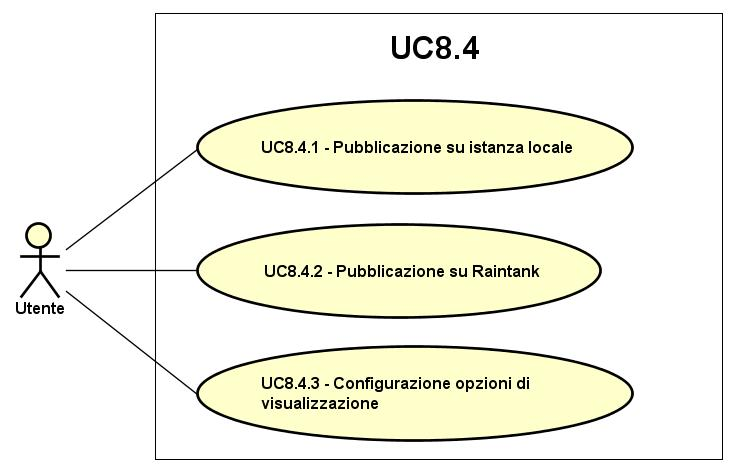
\includegraphics[scale=0.45]{Img/UC8-4}
	\caption{UC8.4 - Condivisione di snapshot}\label{}
\end{figure}
\begin{itemize}
	\item \textbf{Attori}: Utente;
	\item \textbf{Descrizione}: l'attore condivide lo snapshot della dashboard o di un panel e ne configura le opzioni di visualizzazione;
	\item \textbf{Precondizione}: il sistema permette la condivisione di snapshot;
	\item \textbf{Flusso principale degli eventi}:
	\begin{itemize}
		\item Pubblicazione su istanza locale (UC8.4.1);
		\item Pubblicazione su Raintank (UC8.4.2).
	\end{itemize}
	\item \textbf{Postcondizione}: lo snapshot con le relative opzioni di visualizzazione è stato condiviso dall'attore;
	\item \textbf{Estensioni}:
	\begin{itemize}
		\item Configurazione opzioni di visualizzazione (UC8.4.3).
	\end{itemize}
\end{itemize}

\subsection{UC8.4.1: Pubblicazione su istanza locale}
\hypertarget{UC8.4.1}{}
\begin{itemize}
	\item \textbf{Attori}: Utente;
	\item \textbf{Descrizione}: l'attore pubblica lo snapshot della dashboard o di un panel sulla sua istanza locale;
	\item \textbf{Precondizione}: il sistema permette la pubblicazione di snapshot sull'istanza di un utente;
	\item \textbf{Postcondizione}: lo snapshot è stato pubblicato sull'istanza.
\end{itemize}

\subsection{UC8.4.2: Pubblicazione su Raintank}
\hypertarget{UC8.4.2}{}
\begin{itemize}
	\item \textbf{Attori}: Utente;
	\item \textbf{Descrizione}: l'attore pubblica lo snapshot della dashboard o di un panel sulla piattaforma \gl{Raintank};
	\item \textbf{Precondizione}: il sistema permette la pubblicazione di snapshot su Raintank;
	\item \textbf{Postcondizione}: lo snapshot è stato pubblicato su Raintank.
\end{itemize}

\subsection{UC8.4.3: Configurazione opzioni di pubblicazione}
\hypertarget{UC8.4.3}{}
\begin{figure} [H]
	\centering
	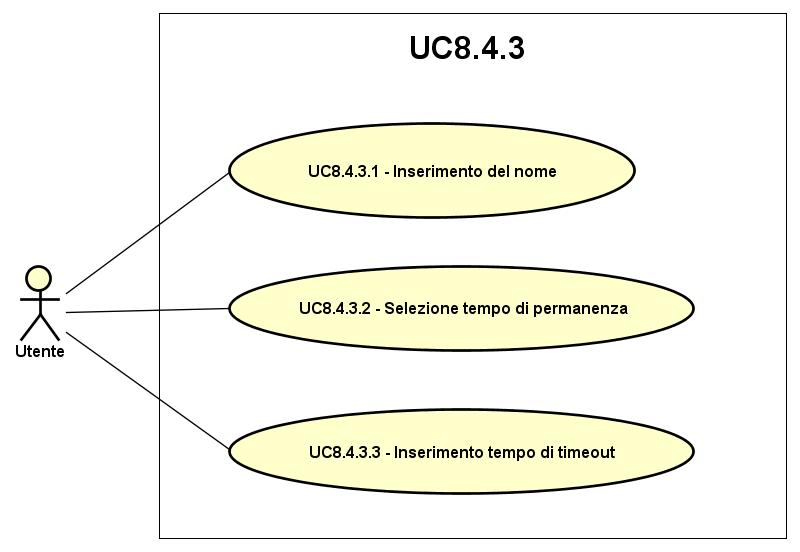
\includegraphics[scale=0.45]{Img/UC8-4-3}
	\caption{UC8.4.3 - Configurazione opzioni di pubblicazione}\label{}
\end{figure}
\begin{itemize}
	\item \textbf{Attori}: Utente;
	\item \textbf{Descrizione}: l'attore configura le opzioni per la pubblicazione dello snapshot della dashboard o di un panel;
	\item \textbf{Precondizione}: il sistema permette di configurare le opzioni per la pubblicazione di snapshot;
	\item \textbf{Flusso principale degli eventi}:
	\begin{itemize}
		\item Inserimento del nome (UC8.4.3.1);
		\item Selezione tempo di permanenza (UC8.4.3.2);
		\item Inserimento tempo per timeout (UC8.4.3.3).
	\end{itemize}
	\item \textbf{Postcondizione}: le opzioni per la pubblicazione dello snapshot sono state configurate.
\end{itemize}

\subsection{UC8.4.3.1: Inserimento del nome}
\hypertarget{UC8.4.3.1}{}
\begin{itemize}
	\item \textbf{Attori}: Utente;
	\item \textbf{Descrizione}: l'attore inserisce il nome dello snapshot;
	\item \textbf{Precondizione}: il sistema permette l'inserimento del nome di uno snapshot;
	\item \textbf{Postcondizione}: il nome dello snapshot è stato inserito.
\end{itemize}

\subsection{UC8.4.3.2: Selezione tempo di permanenza}
\hypertarget{UC8.4.3.2}{}
\begin{itemize}
	\item \textbf{Attori}: Utente;
	\item \textbf{Descrizione}: l'attore seleziona il tempo di permanenza di uno snapshot dal momento della sua pubblicazione;
	\item \textbf{Precondizione}: il sistema permette di selezionare il tempo di permanenza di uno snapshot tra le opzioni predefinite;
	\item \textbf{Postcondizione}: il tempo di permanenza dello snapshot è stato selezionato.
\end{itemize}

\subsection{UC8.4.3.3: Inserimento tempo di timeout}
\hypertarget{UC8.4.3.3}{}
\begin{itemize}
	\item \textbf{Attori}: Utente;
	\item \textbf{Descrizione}: l'attore inserisce il tempo(in secondi) massimo per il caricamento dei dati nello snapshot;
	\item \textbf{Precondizione}: il sistema permette l'inserimento del tempo massimo per il caricamento dei dati di uno snapshot;
	\item \textbf{Postcondizione}: il tempo di timeout è stato inserito.
\end{itemize}

\pagebreak




